\documentclass[a4paper, 11pt]{article}
\usepackage{float}
\usepackage{amsmath}
\usepackage{graphicx}
\usepackage[portuges]{babel}
\usepackage[utf8x]{inputenc}
\usepackage{comment}
\usepackage{fullpage}
\usepackage{xcolor}
\usepackage{multirow}
\usepackage{graphicx}
\usepackage{tabularx}

\usepackage{listings}
\usepackage{color}
\definecolor{mygreen}{RGB}{28,172,0}
\definecolor{mylilas}{RGB}{170,55,241}


\begin{document}
\noindent
\large\textbf{Lista de Exercícios 1} \hfill \textbf{Luis Vinicius Costa Silva} \\
\normalsize Sistemas Bio-Inspirados \\
Prof. Fran Sérgio Lobato \\
\hfill Data de Entrega: 13/04/2019

\section*{Questão 1}
Os dados da tabela resultam da análise de sensibilidade do valor da função objetivo no ponto mínimo computado pelo algoritmo genético. O problema de otimização se encontra abaixo:

\begin{equation}
\begin{aligned}
x_1 \sin({4x_1}) + 1 + x_2 \cdot \sin({2x_2}) \\ 
0 \leq x_1 \leq 10 \\
0 \leq x_2 \leq 10
\end{aligned}
\end{equation}

Para cada valor de semente (entre $0$ e $9$), foi avaliada a sensibilidade do algoritmo. Uma vez que um destes parâmetros era variado, assumia-se valores padrão (\textit{default}) para os demais, da seguinte forma:

\begin{itemize}
\item $n_{Ger} \Rightarrow$ Quantidade máxima de gerações (\textit{default=500});
\item $p_M \Rightarrow$ Probabilidade de mutação (\textit{0.1});
\item $p_C \Rightarrow$ Probabilidade de \textit{default=crossover} (\textit{default=0.9});
\item $N \Rightarrow$ Tamanho da População (\textit{default=50});
\end{itemize}

Os dados da tabela abaixo correspondem aos dados obtidos no experimento e estão detalhados no arquivo ``saida.txt". O experimento pode ser replicado executando do script \textit{Python} ``analiseSensibilidade.py".\newline

\begin{table}[H]
\centering
\resizebox{0.895\textwidth}{!}{%
\begin{tabular}{|l|l|l|l|l|l|l|}
\hline
\multirow{2}{*}{Semente} & \multicolumn{3}{l|}{$N$} & \multicolumn{3}{l|}{$n_{Ger}$} \\ \cline{2-7} 
 & 5 & 50 & 100 & 10 & 100 & 1000 \\ \hline
0 & -13,5496 & -16,6893 & -16,6893 & -16,6482 & -16,6893 & -16,6893 \\ \hline
1 & -16,6893 & -16,6893 & -16,6891 & -16,5547 & -16,6893 & -16,6893 \\ \hline
2 & -16,6893 & -16,6893 & -16,6824 & -13,5556 & -16,6893 & -16,6893 \\ \hline
3 & -16,6889 & -16,6893 & -16,6893 & -14,8395 & -16,6893 & -16,6893 \\ \hline
4 & -16,6893 & -16,6893 & -16,6893 & -16,6234 & -16,6893 & -16,6893 \\ \hline
5 & -13,5559 & -16,6893 & -16,6893 & -13,388 & -16,6891 & -16,6893 \\ \hline
6 & -11,9858 & -16,6893 & -16,6893 & -13,4537 & -16,6893 & -16,6893 \\ \hline
7 & -11,9838 & -16,6893 & -16,6893 & -14,9772 & -16,6893 & -16,6893 \\ \hline
8 & -16,6893 & -16,6893 & -16,6893 & -15,0168 & -15,1193 & -16,6893 \\ \hline
9 & -16,6893 & -16,6893 & -16,6893 & -16,2461 & -16,6893 & -16,6893 \\ \hline
Média & -15,12105 & -16,6893 & -16,68859 & -15,13032 & -16,53228 & -16,6893 \\ \hline
Desvio Padrão & 2,09089225199302 & 0 & 0,00217585232342 & 1,34389386386475 & 0,496470569341448 & 0 \\ \hline
\end{tabular}%
}
%\caption{My caption}
\label{my-label}
\end{table}

% Please add the following required packages to your document preamble:
% \usepackage{multirow}
\begin{table}[H]
\centering
\resizebox{0.9\textwidth}{!}{%
\begin{tabular}{|l|l|l|l|l|l|l|}
\hline
\multirow{2}{*}{Semente} & \multicolumn{3}{l|}{$p_C$} & \multicolumn{3}{l|}{$p_M$} \\ \cline{2-7} 
 & 0,5 & 0,7 & 0,9 & 0,01 & 0,05 & 0,1 \\ \hline
0 & -16,6893 & -16,6893 & -16,6893 & -16,6893 & -16,6893 & -16,6893 \\ \hline
1 & -16,6893 & -16,6893 & -16,6893 & -16,6893 & -16,6893 & -16,6893 \\ \hline
2 & -16,6893 & -16,6893 & -16,6893 & -16,6893 & -16,6893 & -16,6893 \\ \hline
3 & -16,6893 & -16,6893 & -16,6893 & -13,5559 & -16,6893 & -16,6893 \\ \hline
4 & -16,6893 & -16,6893 & -16,6893 & -16,6893 & -16,6893 & -16,6893 \\ \hline
5 & -16,6893 & -16,6893 & -16,6893 & -13,5559 & -16,6893 & -16,6893 \\ \hline
6 & -16,6893 & -16,6893 & -16,6893 & -16,6893 & -16,6893 & -16,6893 \\ \hline
7 & -16,6893 & -16,6893 & -16,6893 & -16,6893 & -16,6893 & -16,6893 \\ \hline
8 & -16,6893 & -16,6893 & -16,6893 & -16,6893 & -15,1193 & -16,6893 \\ \hline
9 & -16,6893 & -16,6893 & -16,6893 & -15,1193 & -16,6893 & -16,6893 \\ \hline
Média & -16,6893 & -16,6893 & -16,6893 & -15,90562 & -16,5323 & -16,6893 \\ \hline
Desvio Padrão & 0 & 0 & 0 & 1,33165509782209 & 0,496477592646435 & 0 \\ \hline
\end{tabular}
}
\caption{Avaliação da sensibilidade dos parâmetros dos AG no valor da função objetivo.}
\label{my-label}
\end{table}

Pode-se concluir que a convergência do algoritmo genético é sensível ao tamanho da população, visto que um aumento neste parâmetro tende a causar um decrescimento no desvio padrão da solução computada (ao custo de mais avaliações da função objetivo a cada iteração). Este comportamento é válido também para o parâmetros de probabilidade de crossover e o número de gerações. \newline
No caso do parâmetro de probabilidade de mutação, não se pode afirmar que um aumento tende a causar a convergência para um mínimo local (como a tabela demonstra), visto que algoritmos genéticos com alta taxa de probabilidade de mutação tendem a alterar uma solução aproximada de forma mais frequente, dificultando o processo de convergência (praticamente destruindo a solução aproximada da iteração anterior). Neste experimento em específico, foram usadas probabilidades de mutação baixas ($0.01, 0.05$ e $0.1$), logo este fenômeno não foi notado. \newline
Como se esperava, um aumento da quantidade de gerações tende a aumentar a precisão da solução computada, visto que um aumento no número de gerações implica em mais iterações no qual o algoritmo é capaz de alterar a solução aproximada ,ao custo de uma convergência mais lenta (e em alguns casos desnecessária). \newline
Taxas de crossover altas são mais adequadas para populações pequenas, já que novos indíviduos da população devem ser o mais distinto possíveis da geração anterior, evitando a homogeneidade precoce da população. Populações maiores permitem uma taxa de crossover moderada, permitindo que parte da população menos apta de uma geração anterior sobreviva a fim de garantir uma solução mais exata. Neste experimento a probabilidade de crossover não apresentou impacto na solução. \newline
Dada a natureza estocástica do algoritmo genético, a semente não apresentou impacto significativo na obtenção da solução do problema.\newline


Estes comportamentos podem ser notado nos gráficos abaixo, onde a solução do problema de minimização (média das soluções de cada semente) está em função de cada parâmetro analisado:

      \begin{figure}[H]
        \center{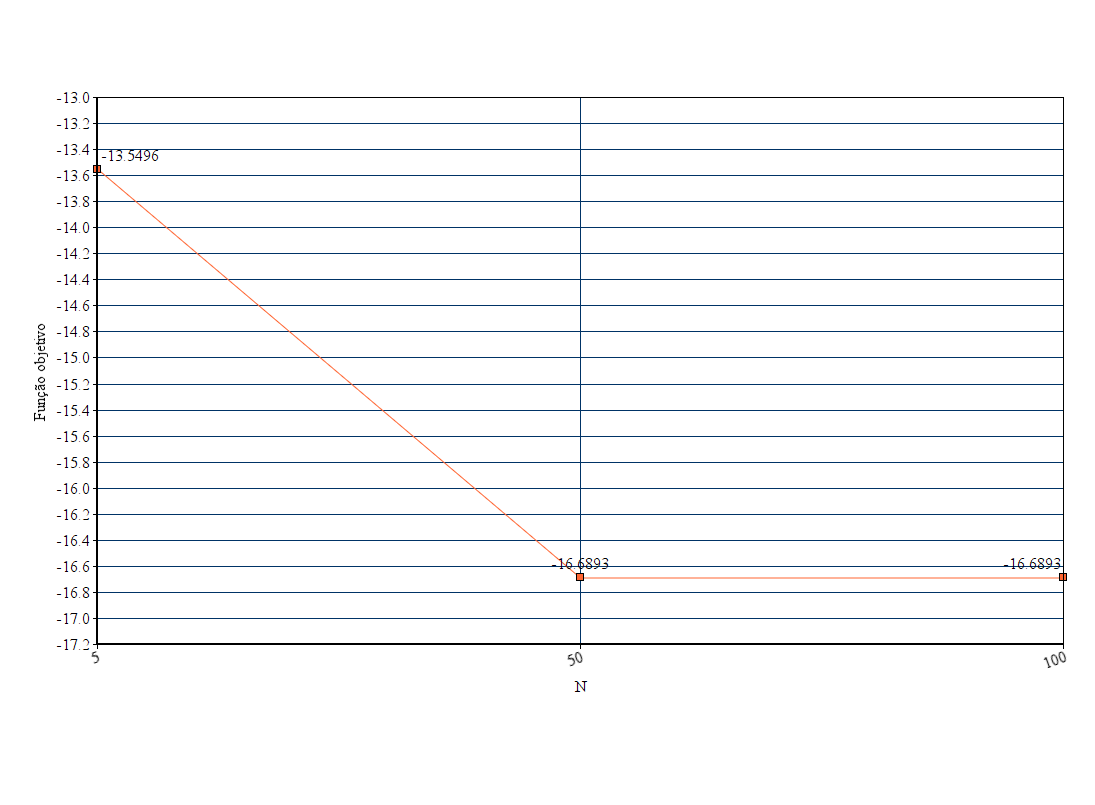
\includegraphics[width=\textwidth]
        {N.png}}
        \caption{\label{fig:my-label} Tamanho da população em função da solução aproximada}
      \end{figure}
 
      \begin{figure}[H]
        \center{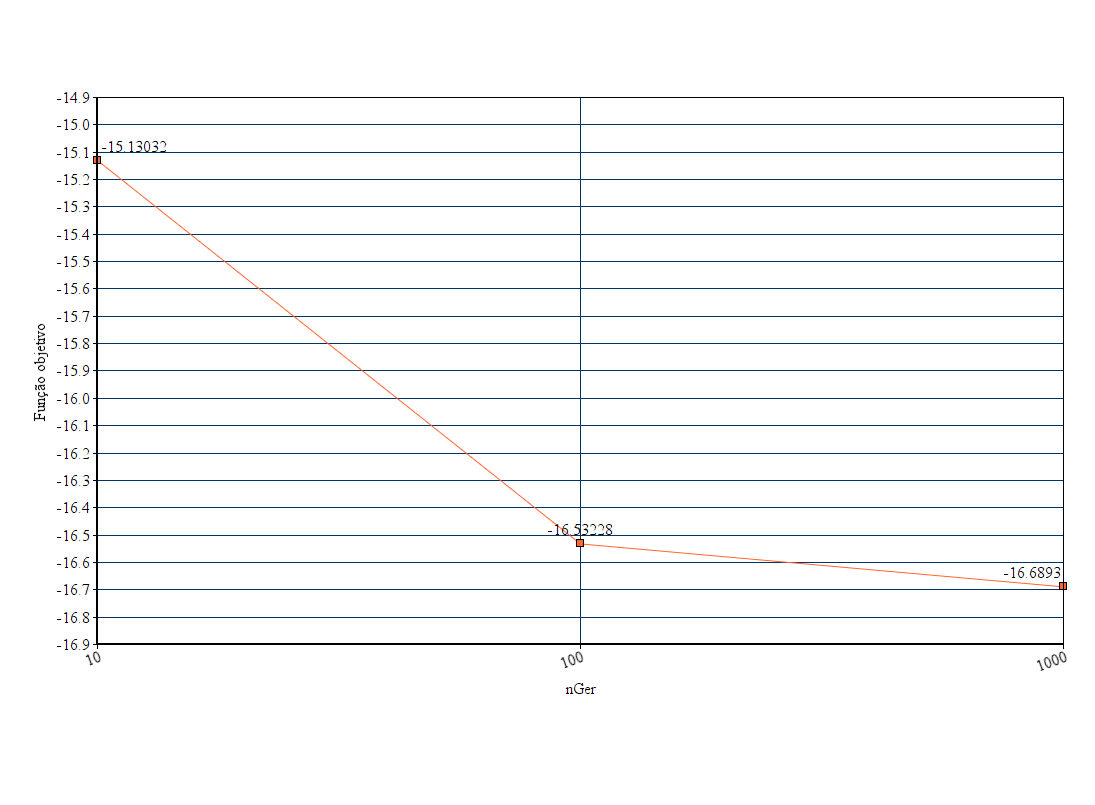
\includegraphics[width=\textwidth]
        {nGer.png}}
        \caption{\label{fig:my-label} Quantidade de gerações em função da solução aproximada}
      \end{figure} 
 
      \begin{figure}[H]
        \center{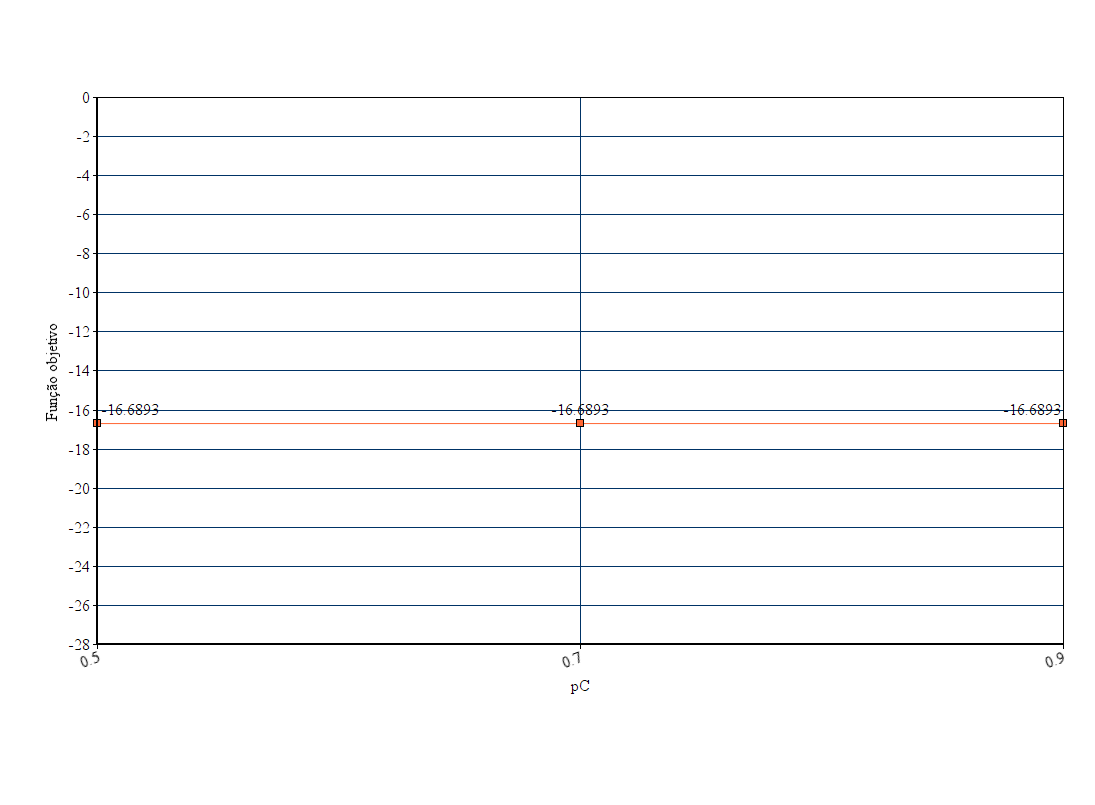
\includegraphics[width=\textwidth]
        {pC.png}}
        \caption{\label{fig:my-label} Probabilidade de crossover em função da solução aproximada}
      \end{figure} 

      \begin{figure}[H]
        \center{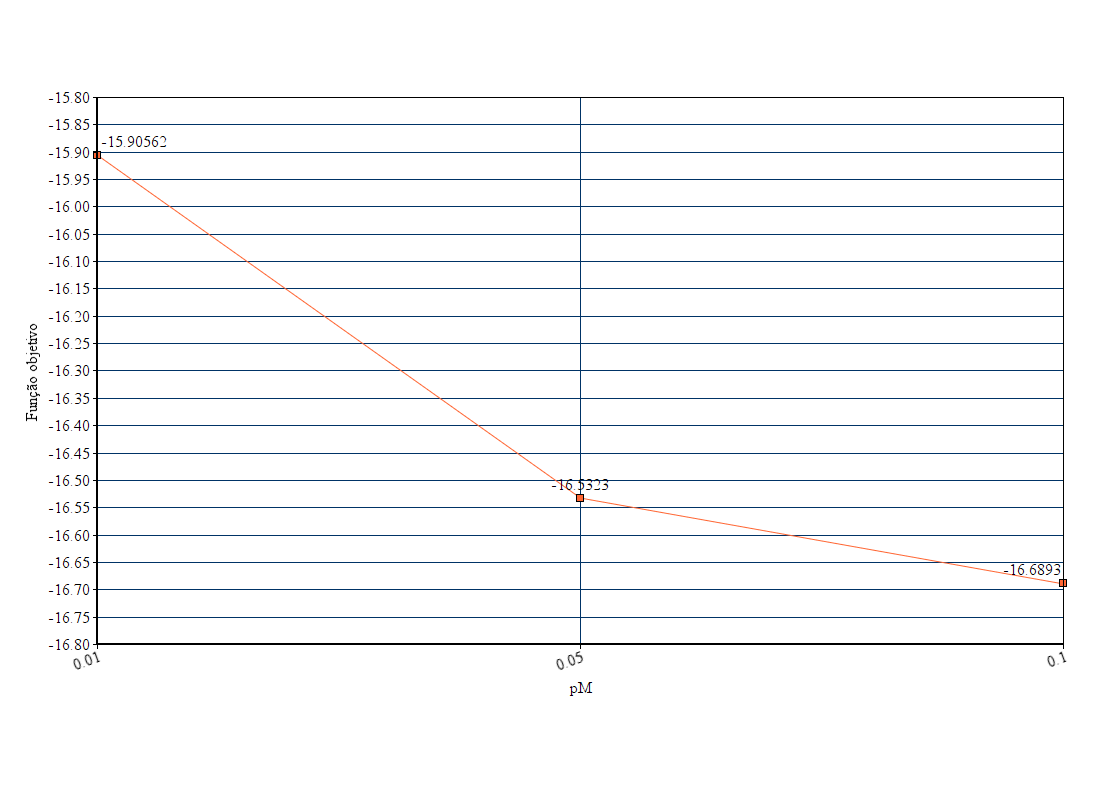
\includegraphics[width=\textwidth]
        {pM.png}}
        \caption{\label{fig:my-label} Probabilidade de mutação em função da solução aproximada}
      \end{figure} 

\section*{Questão 2}
\begin{itemize}
\item Para a análise de um estudo de caso inédito, isto é, você não conhece a solução do problema, o que você
deve fazer para se resguardar quanto ao resultado obtido?
\end{itemize}
Assim como qualquer algoritmo estocástico, algoritmos genéticos (\textit{GA's}) não garantem que um mínimo/máximo global	seja encontrado. Uma técnica que apresenta bons resultados em computar a solução de tais problemas é combinar o GA com a estratégia de recozimento simulado, de tal forma que a taxa de mutação inicial do GA comece com um valor demasiadamente alto, tendo a taxa de mutação reduzida lentamente a cada geração.\newline
Uma vez computado um possível mínimo global, algumas iterações de \textit{Hill Climbing} (ou outro método de otimização clássico) podem ser executadas na vizinha do ponto, possivelmente melhorando o resultado obtido inicialmente.\newline
A execução do GA múltiplas vezes com parâmetros distintos (\textit{tuning}) é essencial em casos onde a solução do problema não é conhecida, neste caso, cada valor de mínimo encontrado deve ser gravado e comparado com os resultados de execuções anteriores. Os critérios de parada recomendados neste caso são:
\begin{itemize}
\item Quantidade máxima de gerações;
\item Solução constante (ou quase) após um número determinado de gerações;
\item O diâmetro da população é suficientemente pequeno (a população convergiu para uma determinada solução).
\end{itemize}
Um estudo do comportamento da função objetivo e do problema em questão são importantes, antes de qualquer tentativa de otimização.
\end{document}